\documentclass[paper=a4, fontsize=11pt]{article}
\usepackage[utf8]{inputenc}
\usepackage[english,magyar]{babel}
\usepackage{amsmath}
\usepackage{graphicx} 
\usepackage{float}
\usepackage{rotating}
\usepackage{latexsym}
\usepackage{listings}

\addtolength{\oddsidemargin}{-.875in}
\addtolength{\evensidemargin}{-.875in}
\addtolength{\textwidth}{1.95in}
\addtolength{\topmargin}{-.9in}
\addtolength{\textheight}{1.6in}

\begin{document}
\begingroup
	\centering
	\LARGE Szimuláció 2: Ising model\\
\vspace{1 cm}
\large Nagy Péter\\
\large M07ILF\\
\vfill
\large 2018.04.09.\\

\newpage

\tableofcontents
\newpage


\section{Mérések}
A mérés során a mellékelt forráskód segítségével 4 különbőző paraméter esetében vizsgáltam a sztohasztikus rendszer viselkedését. A szimulált rendszer egy-dimenziós Ising modellre vonatkozott, ahol az N darab rácspontban $\pm 1$ értékű spinek találhatók. A spinek energiáját a következő képlet adja meg:
\begin{align}
E(s_1,s_2,....s_N)=-J\sum_{1}^{N-1}s_i s_{i+1}
\end{align} 
\newline
\flushleft
 A szimuláció paraméterei:

\begin{itemize}
  \item lépések száma: 10000
\end{itemize}
  



\subsection{Mágnesezetség}
A szimuláciokat elég ideig futatve feltételezhetjük, hogy egyensúlyhoz relakszált a rendszer, így mérhetjük a mágnesezetséget. A fekete oszlopok a kezdeti eloszlást, a piros oszlopok a forgatás utáni eloszlását mutatják a spineknek. Azt figyelhetjük meg, hogy ahogyan növeljük $\beta$ értékét úgy egyre inkább egyenletesen fognak eloszlani a spinek. Ezt azzal lehet magyarázni, hogy az algoritmusban a magas energiájú pontok, ahol több spin azonos irányba néz, inkább tudnak átfordulni és a megadott paraméternek a növelésével kisebb valószinüséget engedünk a spontán átfogásnak mivel az exponens tag értéke csökken és ezzel álítjuk a küszöböt.

\begin{align}
&m=\frac{1}{N}\sum_i^N s_i\\
&<m>=<s_i>
&<m^2>=<s_i^2>
\end{align}



\begin{figure}[H]
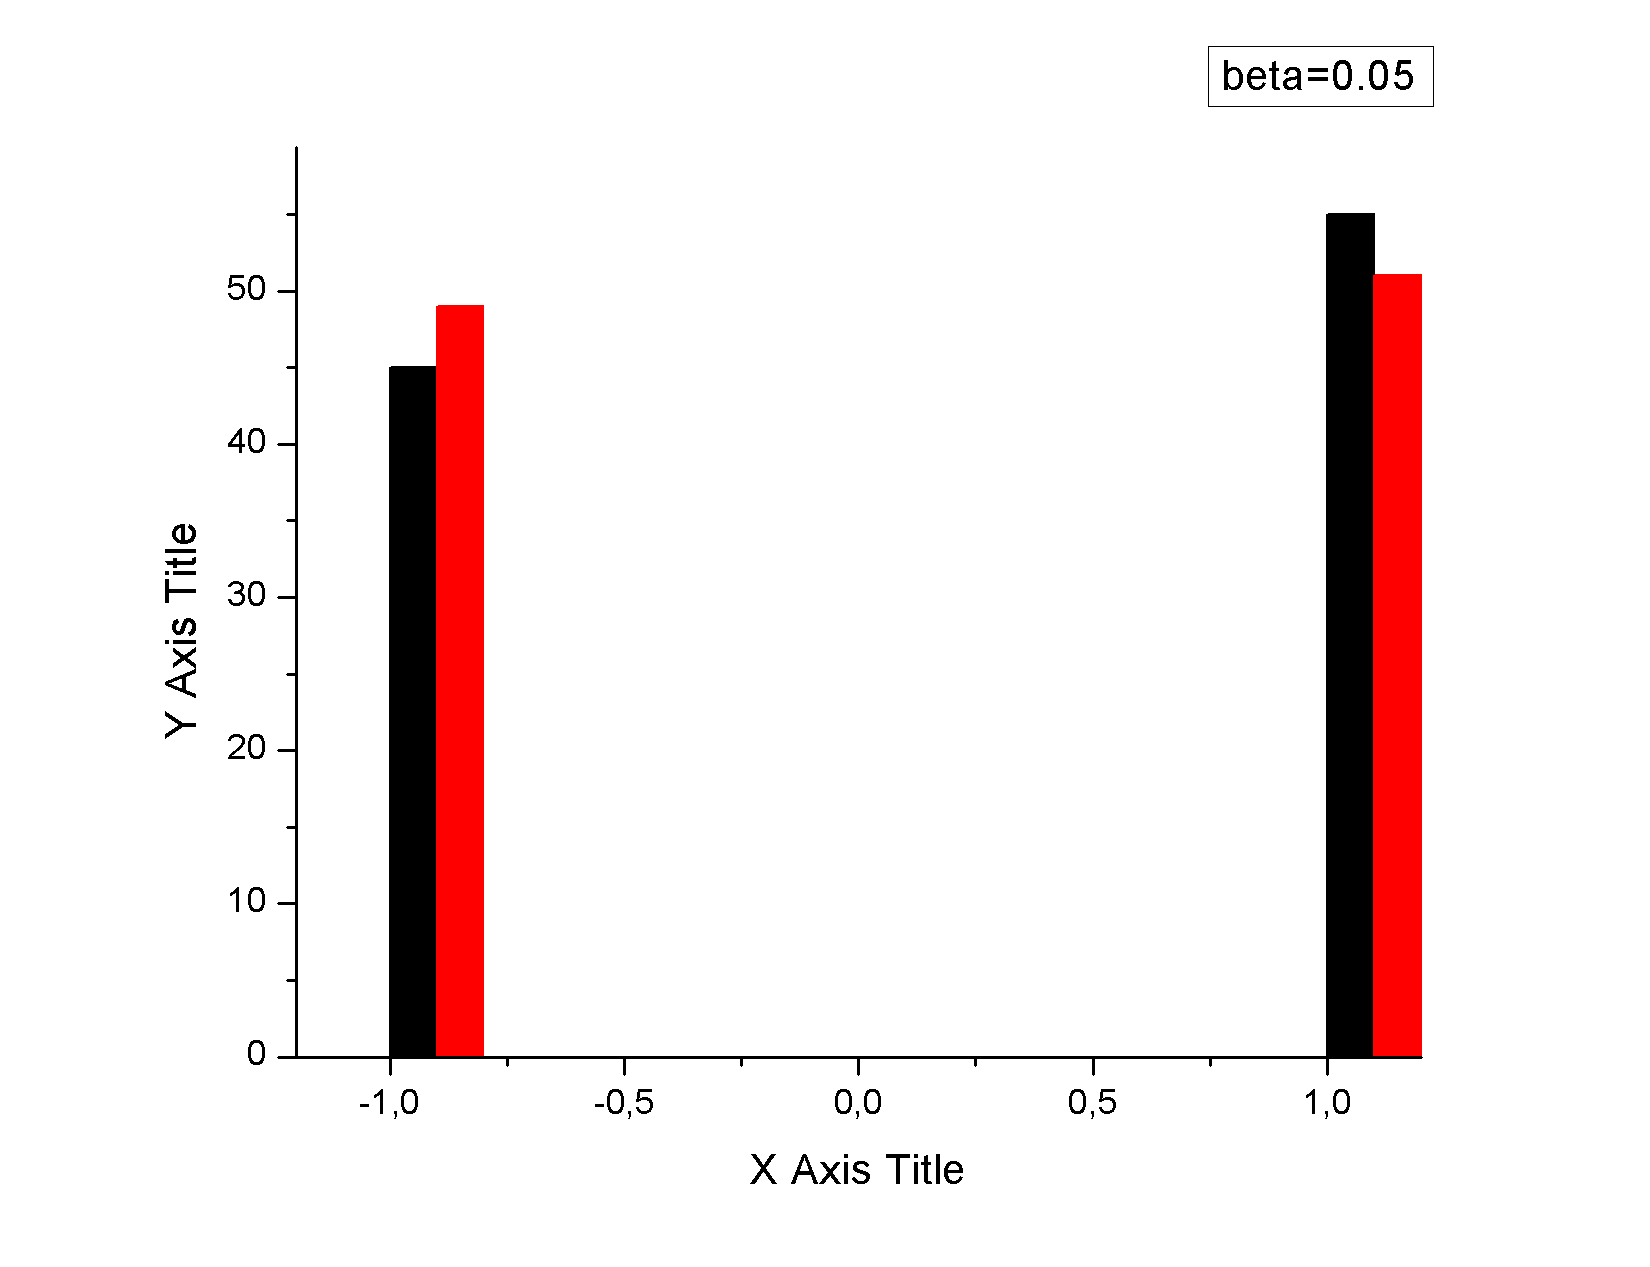
\includegraphics[width=\textwidth]{005}
\caption{Az elfoglalt helyzetek eloszlása}
\end{figure}

\begin{align}
&<m>=0.02\\
&<m^2>=1
\end{align}


\begin{figure}[H]
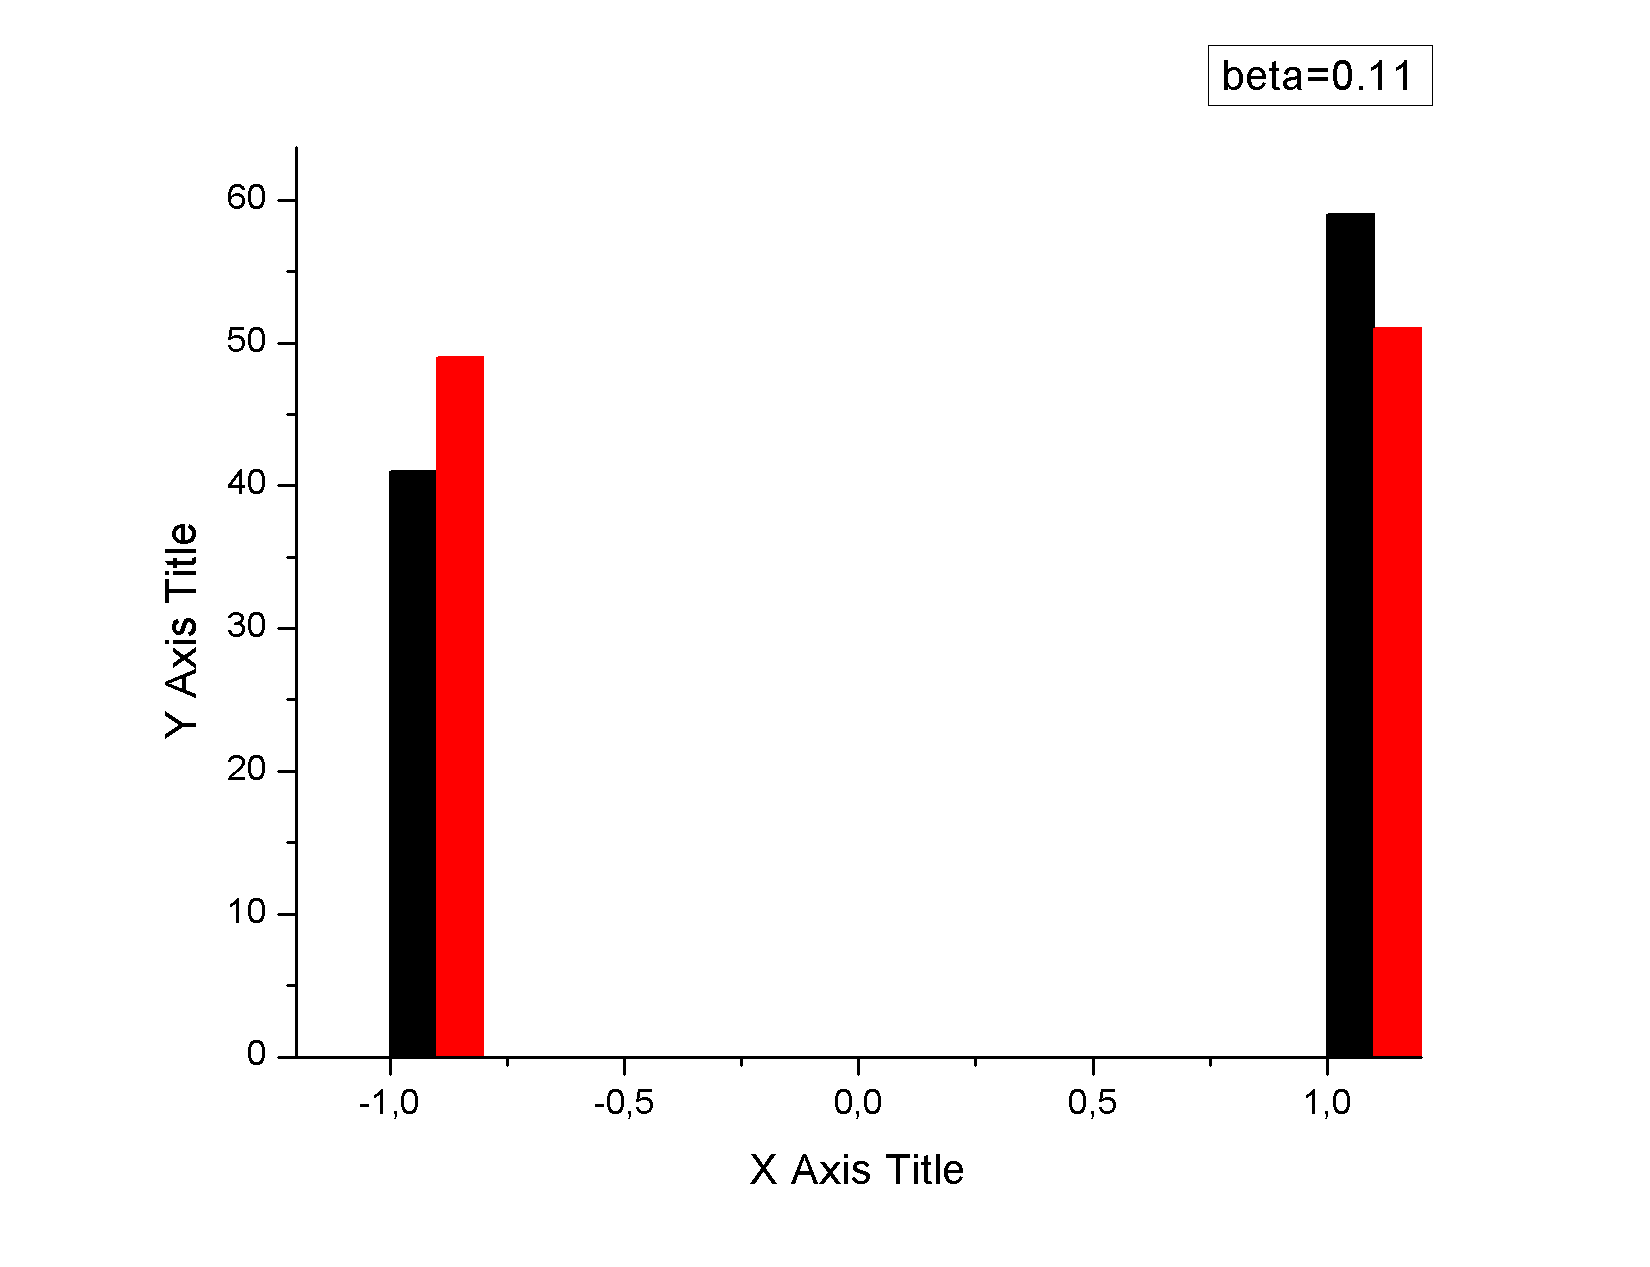
\includegraphics[width=\textwidth]{011}
\caption{Az elfoglalt helyzetek eloszlása}
\end{figure}

\begin{align}
&<m>=-0.02\\
&<m^2>=1
\end{align}



\begin{figure}[H]
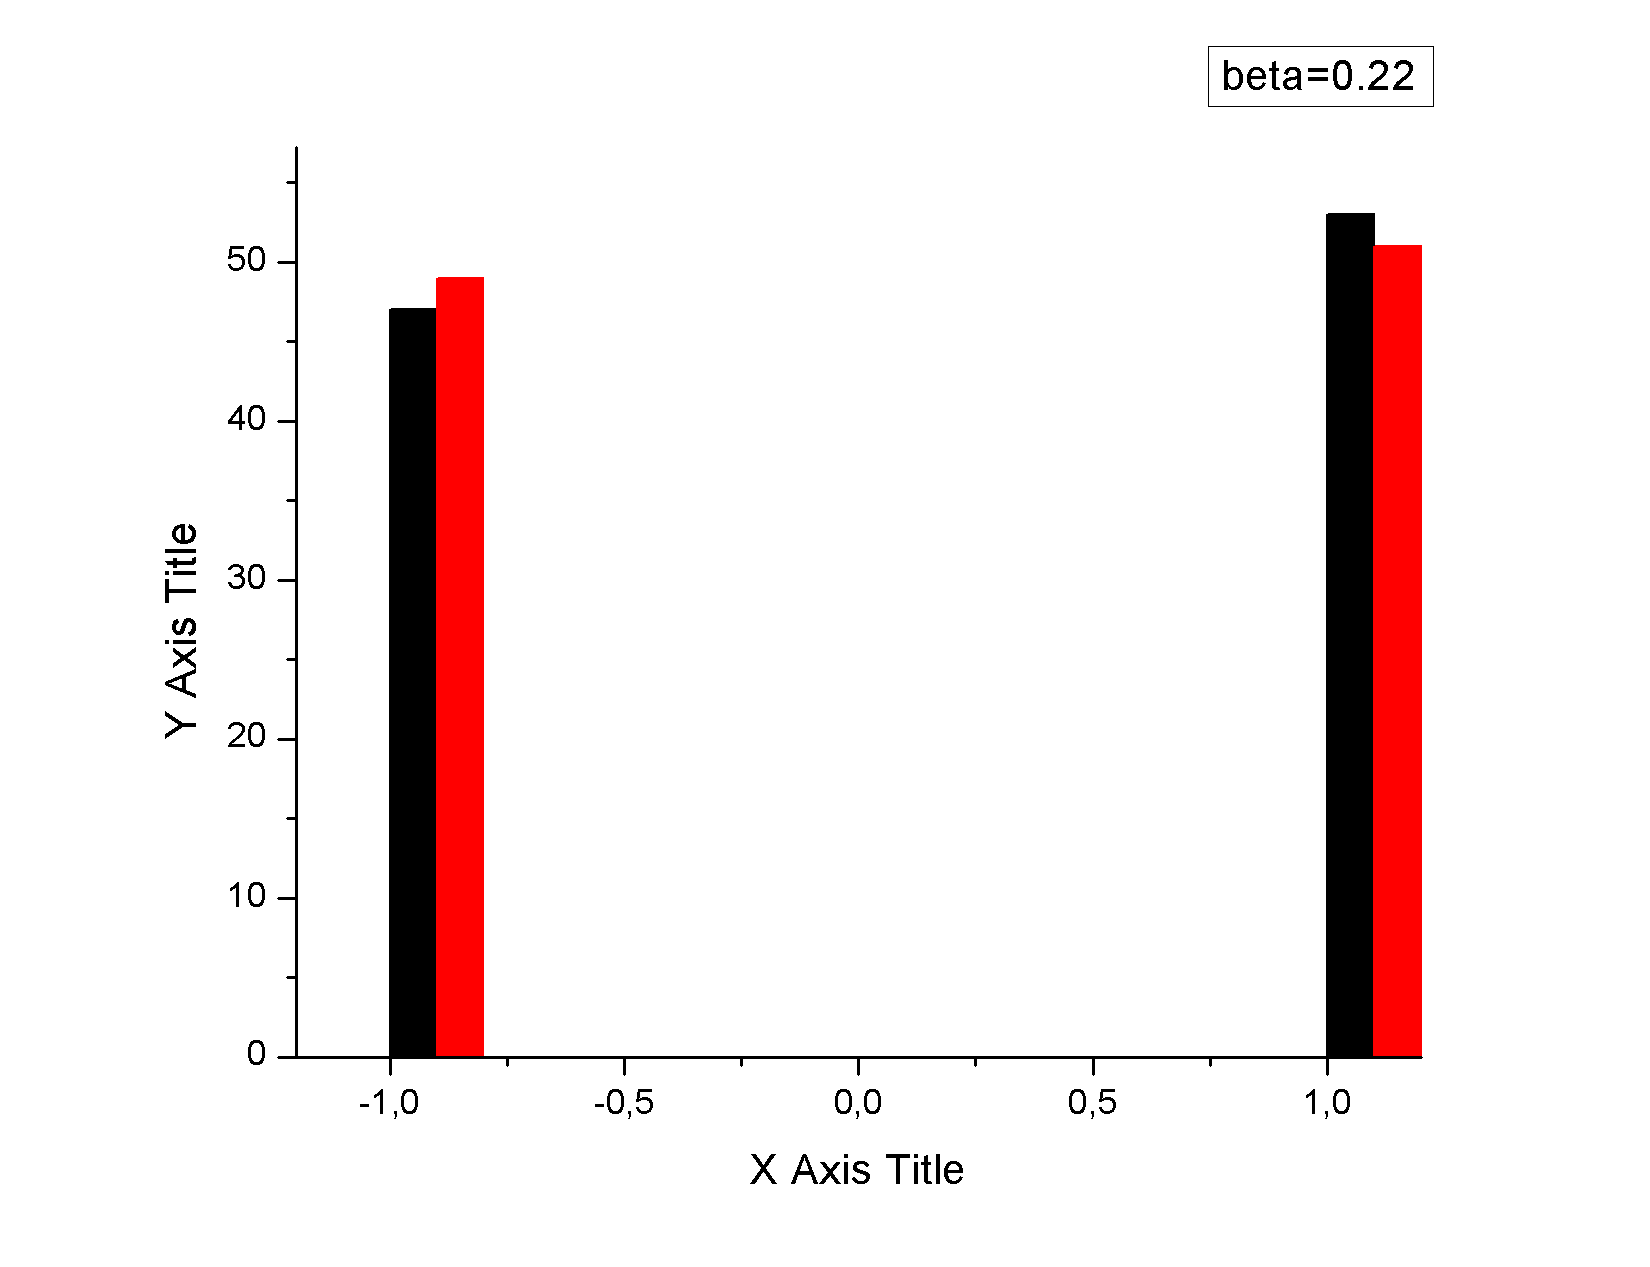
\includegraphics[width=\textwidth]{022}
\caption{Az elfoglalt helyzetek eloszlása}
\end{figure}

\begin{align}
&<m>=0.02\\
&<m^2>=1
\end{align}



\begin{figure}[H]
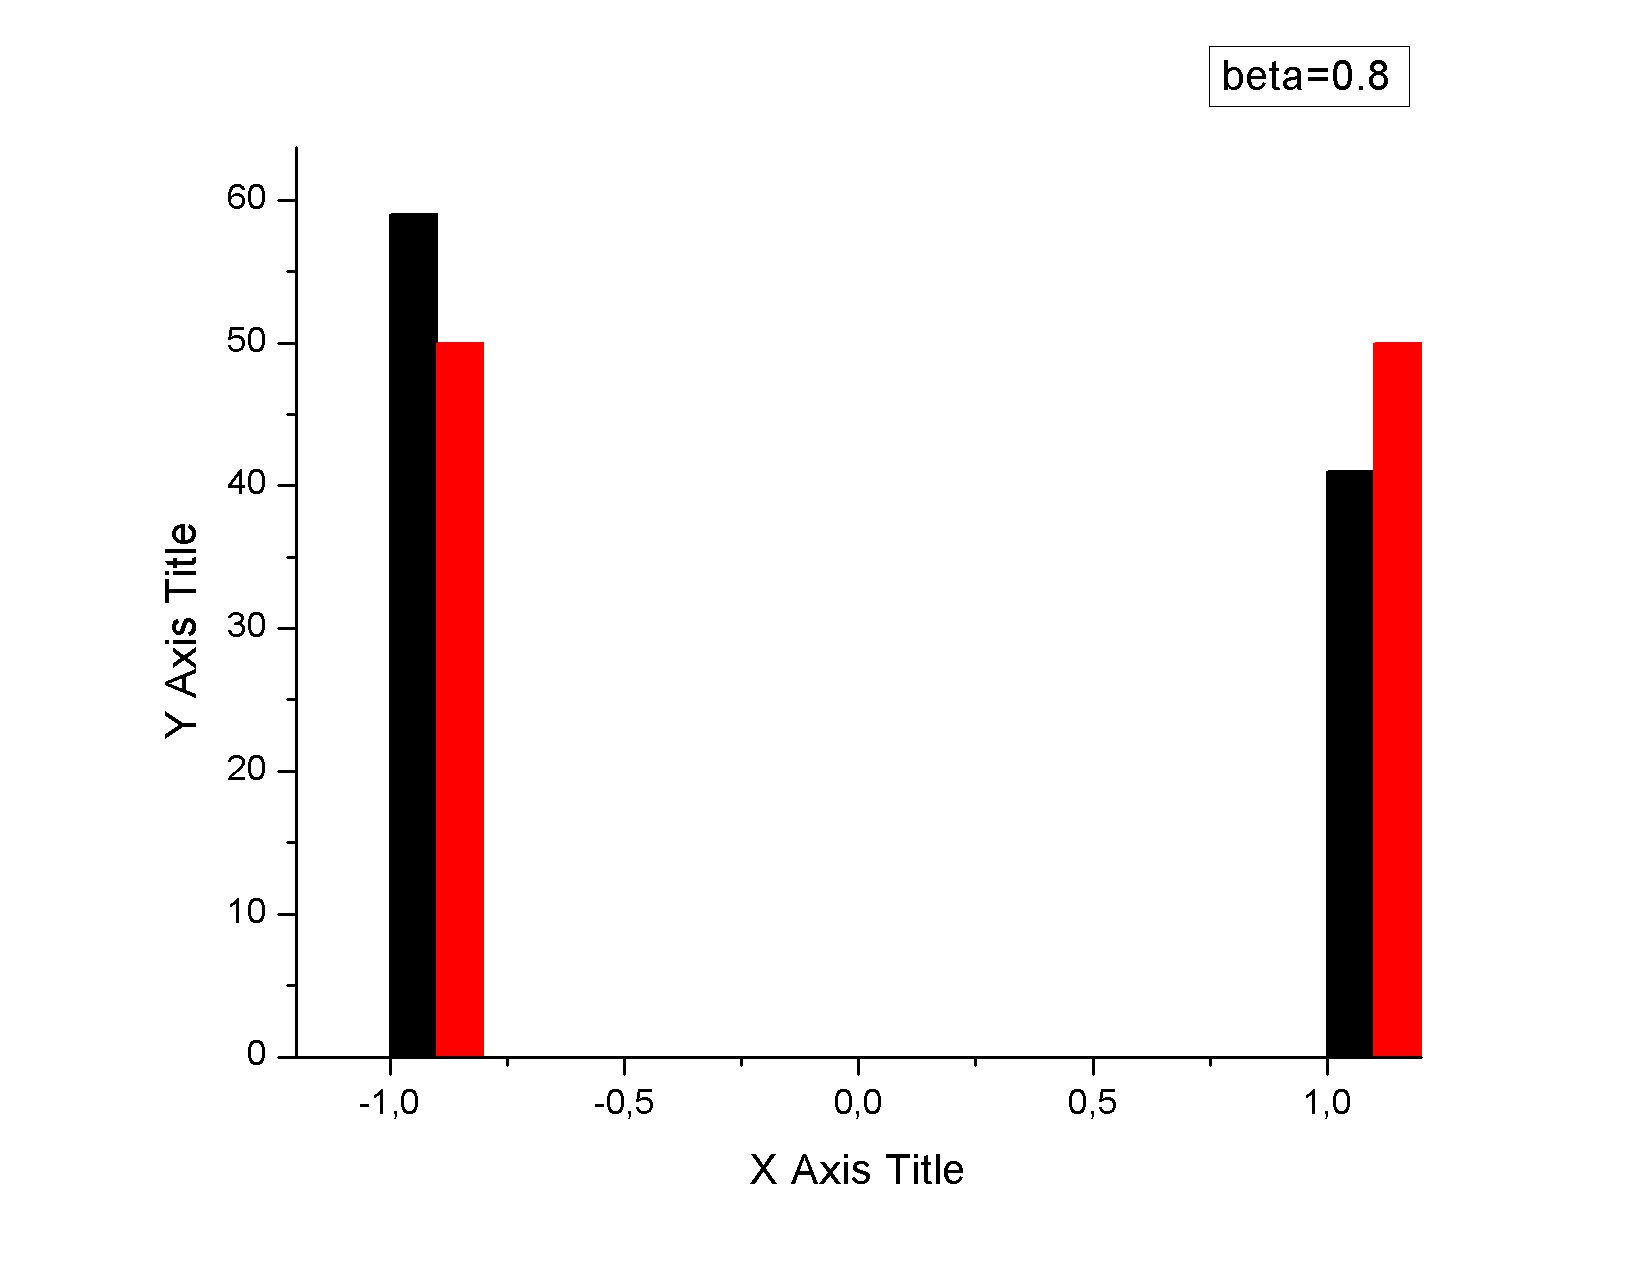
\includegraphics[width=\textwidth]{08}
\caption{Az elfoglalt helyzetek eloszlása}
\end{figure}


\begin{align}
&<m>=0\\
&<m^2>=1
\end{align}


\newpage
\section{A mérés hibája}
A szimuláció statisztikus hibáját egy esetben vizsgáltam $(\beta=0.05)$ majd ezt az értéket általánosnak tekintettem.
\newline
A megismételt mérésekre kapott $<m>$:
\begin{itemize}
  \item 0.02
  \item -0.02
  \item 0
  \item -0.02
  \item -0.02
  \item 0
\end{itemize}

A kapott hiba: $\pm 0.00857$















\end{document}